\documentclass{beamer}

\usepackage{hyperref}
\usepackage{amsfonts}
\usepackage{listings}
%\usepackage{cite}

\usepackage[backend=biber]{biblatex}
\bibliography{bib.bib}

%\setbeamertemplate{bibliography item}{}

\begin{document}

\title{Introduction to CSP}   
\author{Otto Kohul\'{a}k \newline kohulak@fmph.uniba.sk} 
\date{\today} 

\frame{\titlepage} 

\begin{frame}
  \frametitle{What is Crystal Structure prediction?}
  \begin{itemize}
    \item It is searching for stable or metastable crystal structure at given thermodynamic conditions.
    \item Or searching for local extrem in some thermodynamic potential (e.g. Gibbs: $ G = E(\mathbb{X}) + pV(\mathbb{X}) - TS(\mathbb{X}) $).
    \item It is a great tool to propose new structures prior to be found by expensive experiments.
    \item Good book\cite{oganov2011}.
  \end{itemize}
\end{frame}

\begin{frame}
  \frametitle{Order parameters}
  \begin{itemize}
    \item Unit cell (9 parameters in general) + basis (3 * N parameters in general).
    \item If we consider translation a rotational invariance of Hamiltonian (3 * N + 3 parameters).
    \item Other constraints such as minimum distance parametrization \cite{pauschenwein2009}.
  \end{itemize}
\end{frame}

\begin{frame}
  \frametitle{Born - Oppenheimer surface}
  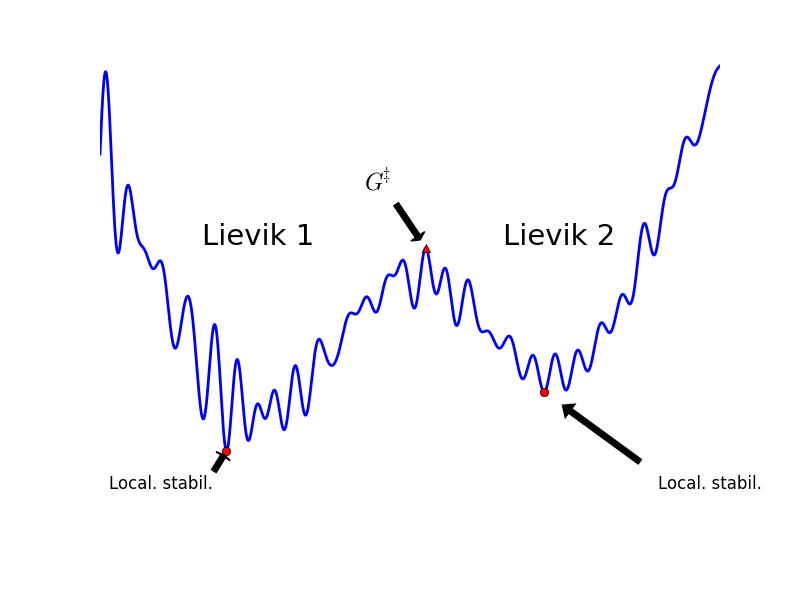
\includegraphics[width=\textwidth]{figs/Lievik.png}
\end{frame}

\begin{frame}
  \frametitle{CSP methods}
  \begin{itemize}
    \item Direct search
    \item Simulated Annealing
    \item Evolutionary algorithms
    \item Particle swarm optimization
    \item Metadynamics
    \item Minima hopping method
    \item Basin hopping method
    \item Periodic-graph approach
  \end{itemize}
\end{frame}

\begin{frame}
  \frametitle{Direct search}
  \begin{itemize}
    \item Very simple method, based on relative easyness of gradient optimization of crystals
    \item Known also as stochastic gradient search
    \item Usefull up to 12 atoms per unit cell
  \end{itemize}
  \centering
  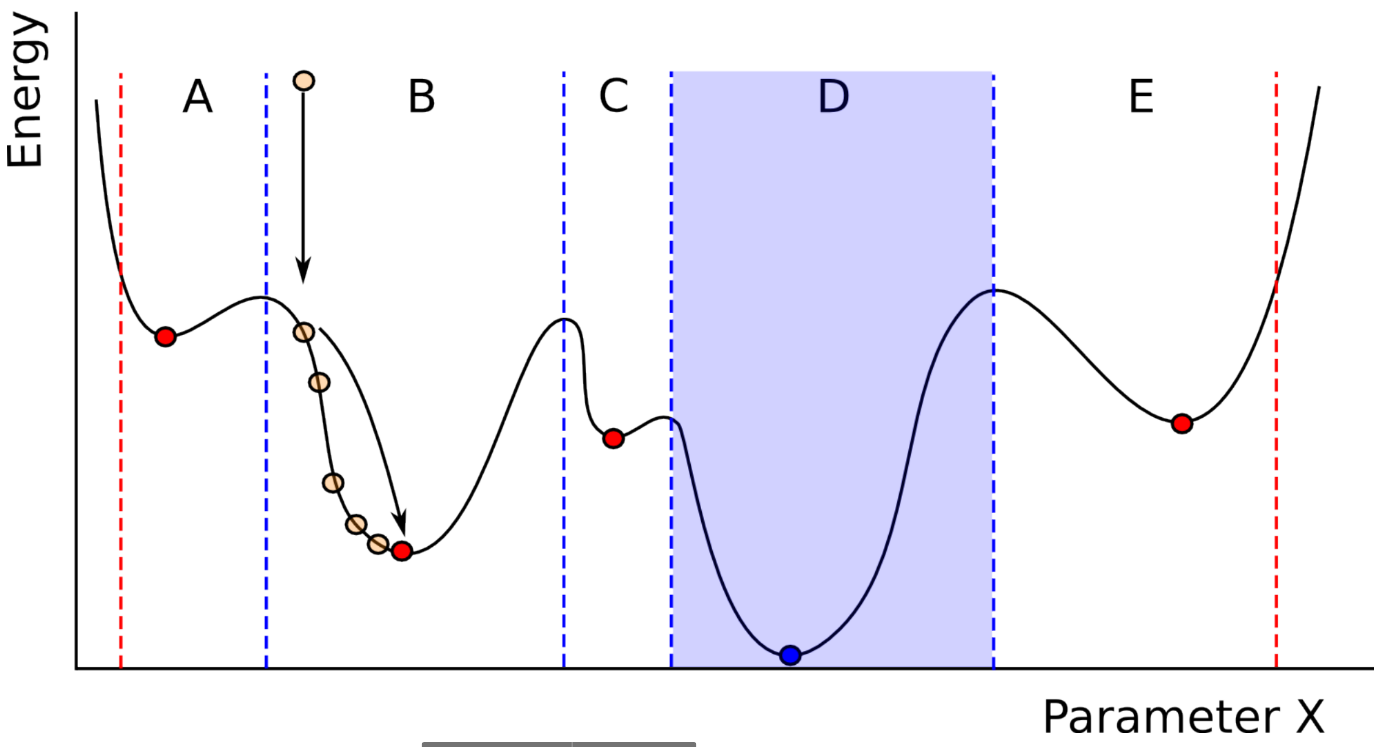
\includegraphics[width=0.7\textwidth]{figs/Priame.png}
\end{frame}

\begin{frame}
  \frametitle{Evolutionary algorithms}
  \begin{minipage}[h]{0.49\textwidth}
    \begin{itemize}
      \item Method inspired by evolution.
      \item Curently one of the most widely used method
      \item Usefull up to 1000 atoms per unit cell
    \end{itemize}
  \end{minipage}%
  \hfill%
  \begin{minipage}[h]{0.49\textwidth}
    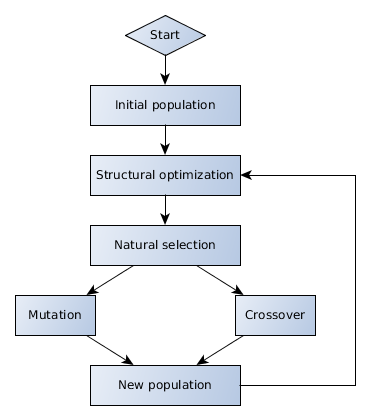
\includegraphics[width=\textwidth]{figs/EA.png}
  \end{minipage}
\end{frame}

\begin{frame}
  \frametitle{References}
  \printbibliography
\end{frame}


\end{document}

